

%\subsection{Couleurs}
%
%
%\subsubsection{Couleurs de base }
\SbSSCT{Couleurs de base }{Basic colors}

\begin{tabular}{|c|c|c|c|c|} \hline
\fbox{\tikz \fill [black] (0,0)rectangle (2,1);}
&
\fbox{\tikz \fill [blue] (0,0)rectangle (2,1);}
&
\fbox{\tikz \fill [brown] (0,0)rectangle (2,1);}
&
\fbox{\tikz \fill [cyan] (0,0)rectangle (2,1);}
&
\fbox{\tikz \fill [darkgray] (0,0)rectangle (2,1);}
\\ \hline 
black & blue &  brown & cyan & darkgray
\\ \hline 
\fbox{\tikz \fill [gray] (0,0)rectangle (2,1);}
&  
\fbox{\tikz \fill [green] (0,0)rectangle (2,1);}
&
\fbox{\tikz \fill [lightgray] (0,0)rectangle (2,1);}
&
\fbox{\tikz \fill [lime] (0,0)rectangle (2,1);}
&
\fbox{\tikz \fill [magenta] (0,0)rectangle (2,1);}
\\ \hline 
gray & green &  lightgray & lime & magenta
\\ \hline 
\fbox{\tikz \fill [olive] (0,0)rectangle (2,1);}
&
\fbox{\tikz \fill [orange] (0,0)rectangle (2,1);}
&
\fbox{\tikz \fill [pink] (0,0)rectangle (2,1);}
&
\fbox{\tikz \fill [purple] (0,0)rectangle (2,1);}
&
\fbox{\tikz \fill [red] (0,0)rectangle (2,1);}
\\ \hline  
olive & orange & pink & purple & red
\\ \hline 
\fbox{\tikz \fill [teal] (0,0)rectangle (2,1);}
&
\fbox{\tikz \fill [violet] (0,0)rectangle (2,1);}
&
\fbox{\tikz \fill [white] (0,0)rectangle (2,1);}
&
\fbox{\tikz \fill [yellow] (0,0)rectangle (2,1);}
&
\\ \hline 
teal & violet & white & yellow &
\\ \hline 
\end{tabular} 

\bigskip

\noindent
\begin{tabular}{|c|c|c|c|c|} \hline  
\fbox{
\begin{tikzpicture}[baseline=-.5]
 \fill [blue!10](0,0)rectangle (2,1);
 \end{tikzpicture}}
& 
\fbox{
\begin{tikzpicture}[baseline=-.5]
 \fill [blue!30](0,0)rectangle (2,1);
 \end{tikzpicture}}
 & 
\fbox{
\begin{tikzpicture}[baseline=-.5]
 \fill [blue!50](0,0)rectangle (2,1);
  \end{tikzpicture}}
   & 
  \fbox{
\begin{tikzpicture}[baseline=-.5]
   \fill [blue!70](0,0)rectangle (2,1);
    \end{tikzpicture}}
      & 
     \fbox{
\begin{tikzpicture}[baseline=-.5]
      \fill [blue!70](0,0)rectangle (2,1);
       \end{tikzpicture}}
 \\ 
\hline [blue!10]  & [blue!30] &[blue!50] & [blue!70] & [blue!90]\\ 
\hline 
\end{tabular}
  
%\subsubsection{Mélange de couleurs}
\SbSSCT{Mélange de couleurs}{Colors mixing}


\begin{tabular}{|c|c|c|c|} \hline  
\fbox{
\begin{tikzpicture}[baseline=-.5]
 \fill [blue!30!red](0,0)rectangle (2,1);
 \end{tikzpicture}}
& 
\fbox{
\begin{tikzpicture}[baseline=-.5]
 \fill [red!80!blue!20](0,0)rectangle (2,1);
 \end{tikzpicture}}
 & 
\fbox{
\begin{tikzpicture}[baseline=-.5]
 \fill [red!80!blue!50](0,0)rectangle (2,1);
  \end{tikzpicture}}
   & 
  \fbox{
\begin{tikzpicture}[baseline=-.5]
   \fill [red!80!blue!50!black!40](0,0)rectangle (2,1);
    \end{tikzpicture}}
 \\ 
\hline [blue!30!red]  & [red!80!blue!20] &[red!80!blue!50] & [red!80!blue!50!black!40] \\ 
\hline 
\end{tabular}
 
 
%%+++++++++++++

%\subsectioa colorn{Créer son nom de couleur}
\SbSSCT{Créer son nom de couleur}{Naming a color}

\begin{center}
\RRR{15-2}
\end{center}

%\subsubsection{A pourcentage de rouge vert et  bleue}
\SbSbSSCT{A pourcentage de rouge vert et  bleue}{Percentage of red , green and blue}


\begin{tabular}{|c|c|} \hline  
\definecolor{macouleur}{rgb}{.75,0.5,0.25}

\fbox{
\begin{tikzpicture}[baseline=-.5]
\fill [macouleur] (0,0)rectangle (2,1);
\end{tikzpicture}}
&  
\parbox[b]{8cm}{
\BSS{definecolor}\AC{{\color{red} macouleur}}\AC{rgb}\AC{.75,0.5,0.25}\\
(75\% de rouge 50\% de vert 25\% de bleu)\\
 \BS{fill} [{\color{red} macouleur}] (0,0) rectangle (2,1);
}
\\ \hline 
\end{tabular} 

%\subsubsection{A partir d'une couleur existante}
\SbSbSSCT{A partir d'une couleur existante}{From existing color}

\begin{tabular}{|c|c|} \hline  
\colorlet{monrouge}{red!25}

\fbox{
\begin{tikzpicture}[baseline=-.5]
 \fill [monrouge] (0,0)rectangle (2,1);
 \end{tikzpicture}} 
&  
\parbox[b]{8cm}{
\BSS{colorlet}\AC{{\color{red} monrouge}}\AC{red!25}
 \\
 \BS{fill} [{\color{red} monrouge}] (0,0) rectangle (2,1);
}
\\ \hline
\colorlet{monviolet}{red!25!blue}
\fbox{
\begin{tikzpicture}[baseline=-.5]
 \fill [monviolet] (0,0)rectangle (2,1);
 \end{tikzpicture}} 
&  
\parbox[b]{8cm}{
\BSS{colorlet}\AC{{\color{red} monviolet}}\AC{red!25!blue}
 \\
 \BS{fill} [{\color{red} monviolet}] (0,0) rectangle (2,1);
}
\\ \hline 
\end{tabular}


%==========================
\newpage

%%\section{Opacité} 
\SSCT{Opacité}{Opacity} 

\begin{center}
\RRR{23-2}
\end{center}

\begin{tabular}{|c|c|c|c|c|} \hline
\multicolumn{5}{|c|}{\BS{draw}[red] (0,0) -- (2,1);\hspace{.5cm} \BS{draw} [blue,\RDD{draw opacity}=0] (0,1) - - (2,0);}
 \\ \hline  

\begin{tikzpicture}[line width=.5cm]
\draw[red] (0,0) -- (2,1);
\draw [blue,draw opacity=0] (0,1) -- (2,0);
\end{tikzpicture}
&  

\begin{tikzpicture}[line width=.5cm]
\draw[red] (0,0) -- (2,1);
\draw [blue,draw opacity=0.25] (0,1) -- (2,0);
\end{tikzpicture}
&  
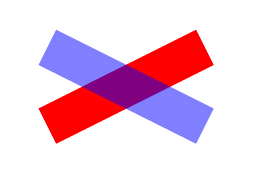
\begin{tikzpicture}[line width=.5cm]
\draw[red] (0,0) -- (2,1);
\draw [blue,draw opacity=0.5] (0,1) -- (2,0);
\end{tikzpicture}
&  

\begin{tikzpicture}[line width=.5cm]
\draw[red] (0,0) -- (2,1);
\draw [blue,draw opacity=0.75] (0,1) -- (2,0);
\end{tikzpicture}
&  

\begin{tikzpicture}[line width=.5cm]
\draw[red] (0,0) -- (2,1);
\draw [blue,draw opacity=1] (0,1) -- (2,0);
\end{tikzpicture}

\\ \hline  
draw opacity=0 & draw opacity=0.25 & draw opacity=0.5 & draw opacity=0.75 & draw opacity=1\\ 
\hline 
\end{tabular} 

\bigskip

\begin{tabular}{|c|c|c|c|} \hline 
\multicolumn{4}{|c|}{\BS{fill}[red] (0,0) rectangle (1,1);\hspace{.5cm} \BS{fill}[blue,\RDD{transparent}] (0.5,0) rectangle (1.5,1);}
 \\ \hline
\fbox{
\begin{tikzpicture}
\fill[red] (0,0) rectangle (1,1);
\fill[blue,transparent] (0.5,0) rectangle (1.5,1);
\end{tikzpicture}}   
&
\fbox{
\begin{tikzpicture}
\fill[red] (0,0) rectangle (1,1);
\fill[blue,ultra nearly transparent] (0.5,0) rectangle (1.5,1);
\end{tikzpicture}}   
&
\fbox{
\begin{tikzpicture}
\fill[red] (0,0) rectangle (1,1);
\fill[blue,very nearly transparent] (0.5,0) rectangle (1.5,1);
\end{tikzpicture}}   

&
\fbox{
\begin{tikzpicture}
\fill[red] (0,0) rectangle (1,1);
\fill[blue,nearly transparent] (0.5,0) rectangle (1.5,1);
\end{tikzpicture}}

\\ \hline  
\RDD{transparent} & \RDD{ultra nearly transparent} & \RDD{very nearly transparent} & \RDD{nearly transparent} \\ 
\hline 
\fbox{
\begin{tikzpicture}
\fill[red] (0,0) rectangle (1,1);
\fill[blue,semitransparent] (0.5,0) rectangle (1.5,1);
\end{tikzpicture}}

&
\fbox{
\begin{tikzpicture}
\fill[red] (0,0) rectangle (1,1);
\fill[blue,nearly opaque] (0.5,0) rectangle (1.5,1);
\end{tikzpicture}}

&
\fbox{
\begin{tikzpicture}
\fill[red] (0,0) rectangle (1,1);
\fill[blue,very nearly opaque] (0.5,0) rectangle (1.5,1);
\end{tikzpicture}}

&
\fbox{
\begin{tikzpicture}
\fill[red] (0,0) rectangle (1,1);
\fill[blue,ultra nearly opaque] (0.5,0) rectangle (1.5,1);
\end{tikzpicture}}

\\ \hline 
\RDD{semitransparent} & \RDD{nearly opaque} & \RDD{very nearly opaque} & \RDD{ultra nearly opaque}
\\ \hline
\fbox{
\begin{tikzpicture}
\fill[red] (0,0) rectangle (1,1);
\fill[blue,opaque] (0.5,0) rectangle (1.5,1);
\end{tikzpicture}} 

&
\fbox{
\begin{tikzpicture}
\fill[red] (0,0) rectangle (1,1);
\fill[blue,fill opacity=.25] (0.5,0) rectangle (1.5,1);
\end{tikzpicture}}
&
\fbox{
\begin{tikzpicture}
\fill[red] (0,0) rectangle (1,1);
\fill[blue,fill opacity=.5] (0.5,0) rectangle (1.5,1);
\end{tikzpicture}}
&
\fbox{
\begin{tikzpicture}
\fill[red] (0,0) rectangle (1,1);
\fill[blue,fill opacity=.75] (0.5,0) rectangle (1.5,1);
\end{tikzpicture}}

\\ \hline 
\RDD{opaque} & \RDD{fill opacity}=.25 & \RDD{fill opacity}=.5 & \RDD{fill opacity}=.75
\\ \hline 
\end{tabular} 

\bigskip


\begin{tabular}{|c|c|c|c|c|} \hline 
\multicolumn{5}{|c|}{\BS{node} at (1,1) [\RDD{text opacity}=1] \AC{ \BS{Huge} texte} ;}
 \\ \hline  
\fbox{\tikz{ %\fill[red] (0,0) rectangle (2,2);
\node at (1,1) [text opacity=1] {\Huge texte} ; }}
&  
\fbox{\tikz{ %\fill[red] (0,0) rectangle (2,2);
\node at (1,1) [text opacity=.75] {\Huge texte} ; }}
&  
\fbox{\tikz{ %\fill[red] (0,0) rectangle (2,2);
\node at (1,1) [text opacity=.5] {\Huge texte} ; }}
&  
\fbox{\tikz{ %\fill[red] (0,0) rectangle (2,2);
\node at (1,1) [draw,text opacity=.25] {\Huge texte} ; }}
&  
\fbox{\tikz{ %\fill[red] (0,0) rectangle (2,2);
\node at (1,1) [draw,text opacity=0] {\Huge texte} ;= }}
\\ \hline  
text opacity=1 & text opacity=0.75 & text opacity=0.5 & opacity=0.25 & text opacity=0 
\\ \hline 
\end{tabular} 

%===============
\newpage

\subsection{Blend Modes} 

\begin{center}
\RRR{23-3} 
\end{center}

\begin{tabular}{|c|c|c|} \hline  
\tikz [blend group=normal] {
\fill[red!50] ( 90:.6) circle (1);
\fill[green!50] (210:.6) circle (1);
\fill[blue!50] (330:.6) circle (1);
}
&  
\tikz [blend group=multiply ] {
\fill[red!50] ( 90:.6) circle (1);
\fill[green!50] (210:.6) circle (1);
\fill[blue!50] (330:.6) circle (1);
}
&  
\tikz [blend group=screen] {
\fill[red!50] ( 90:.6) circle (1);
\fill[green!50] (210:.6) circle (1);
\fill[blue!50] (330:.6) circle (1);
}
\\ \hline 
blend group=\BDD{normal} & blend group=\BDD{multiply} & blend group=\BDD{screen}  
\\ \hline
\tikz [blend group=overlay] {
\fill[red!50] ( 90:.6) circle (1);
\fill[green!50] (210:.6) circle (1);
\fill[blue!50] (330:.6) circle (1);
}
&
\tikz [blend group=darken] {
\fill[red!50] ( 90:.6) circle (1);
\fill[green!50] (210:.6) circle (1);
\fill[blue!50] (330:.6) circle (1);
}
&  
\tikz [blend group=lighten] {
\fill[red!50] ( 90:.6) circle (1);
\fill[green!50] (210:.6) circle (1);
\fill[blue!50] (330:.6) circle (1);
}
\\ \hline 
 blend group=\BDD{overlay} & blend group=\BDD{darken} & blend group=\BDD{lighten} 
\\ \hline    
\tikz [blend group=difference] {
\fill[red!50] ( 90:.6) circle (1);
\fill[green!50] (210:.6) circle (1);
\fill[blue!50] (330:.6) circle (1);}
&  
\tikz [blend group=exclusion] {
\fill[red!50] ( 90:.6) circle (1);
\fill[green!50] (210:.6) circle (1);
\fill[blue!50] (330:.6) circle (1);}
&
\tikz [blend group=hue] {
\fill[red!50] ( 90:.6) circle (1);
\fill[green!50] (210:.6) circle (1);
\fill[blue!50] (330:.6) circle (1);
}
\\ \hline 
 blend group=\BDD{difference} & blend group=\BDD{exclusion} & blend group=\BDD{hue} 
\\ \hline  
\tikz [blend group=saturation] {
\fill[red!50] ( 90:.6) circle (1);
\fill[green!50] (210:.6) circle (1);
\fill[blue!50] (330:.6) circle (1);
}
&  
\tikz [blend group=color] {
\fill[red!50] ( 90:.6) circle (1);
\fill[green!50] (210:.6) circle (1);
\fill[blue!50] (330:.6) circle (1);
}
&  
\tikz [blend group=luminosity] {
\fill[red!50] ( 90:.6) circle (1);
\fill[green!50] (210:.6) circle (1);
\fill[blue!50] (330:.6) circle (1);}
\\ \hline 
 blend group=\BDD{saturation} & blend group=\BDD{color} & blend group=\BDD{luminosity}
\\ \hline 
\end{tabular} 

\bigskip
\begin{tabular}{|c|c|c|c|} \hline
\multicolumn{4}{|c|}{\TFRGB{A revoir message d'erreur}{Error message } Unknow blend mode ! }
\\ \hline  
%\tikz [blend group=colordodge] {
%\fill[red!50] ( 90:.6) circle (1);
%\fill[green!50] (210:.6) circle (1);
%\fill[blue!50] (330:.6) circle (1);
%}
&  
%\tikz [blend group=colorburn] {
%\fill[red!50] ( 90:.6) circle (1);
%\fill[green!50] (210:.6) circle (1);
%\fill[blue!50] (330:.6) circle (1);
%} 

&  
%\tikz [blend group=hardlight] {
%\fill[red] ( 90:.6) circle (1);
%\fill[green] (210:.6) circle (1);
%\fill[blue] (330:.6) circle (1);
%}
&  
%\tikz [blend group=softlight] {
%\fill[red] ( 90:.6) circle (1);
%\fill[green] (210:.6) circle (1);
%\fill[blue] (330:.6) circle (1);
%}
\\ \hline  
blend group=colordodge & blend group=colorburn  & blend group=hardlight & blend group=softlight \\ 
\hline 
\end{tabular} 

\newpage

%==================
\subsection{Fading} 
%Insérer dans le préambule :

 \maboite{\BS{usetikzlibrary}\AC{fadings}}

\label{lib-fadings}

%\subsubsection{Modèles prédéfinis }

\SbSbSSCT{Modèles prédéfinis }{Preset patterns}

\begin{center}
 \RRR{51}
\end{center}
 
\begin{tabular}{|c|c|c|c|} \hline  
\multicolumn{4}{|l|}{ \BS{fill} [blue,\RDD{path fading}=north] (-1,-1) rectangle (1,1);}
\\ \hline
\begin{tikzpicture}
 \draw (-1,-1) rectangle (1,1);
\fill [blue,path fading=north] (-1,-1) rectangle (1,1);
\end{tikzpicture}
&  
\begin{tikzpicture}
 \draw (-1,-1) rectangle (1,1);
\fill [blue,path fading=south] (-1,-1) rectangle (1,1);
\end{tikzpicture}
&  
\begin{tikzpicture}
\draw (-1.2,-1.2) rectangle (1.2,1.2);
\fill [path fading=east] (-1,-1) rectangle (1,1);
\end{tikzpicture} 
& 
\begin{tikzpicture}
\draw (-1.2,-1.2) rectangle (1.2,1.2);
\fill [path fading=west] (-1,-1) rectangle (1,1);
\end{tikzpicture}
\\ \hline  
path fading=north & path fading=south & path fading=east  & path fading=west   
\\ \hline 
\end{tabular}

\begin{tabular}{|c|c|} \hline  
\begin{tikzpicture}
 \draw (-1,-1) rectangle (1,1);
\fill [blue,path fading=circle with fuzzy edge 10 percent] (-1,-1) rectangle (1,1);
\end{tikzpicture}
&
\begin{tikzpicture}
 \draw (-1,-1) rectangle (1,1);
\fill [blue,path fading=circle with fuzzy edge 15 percent] (-1,-1) rectangle (1,1);
\end{tikzpicture}
\\ \hline 
path fading=circle with fuzzy edge 10 percent & path fading=circle with fuzzy edge 15 percent 
\\ \hline 
\begin{tikzpicture}
 \draw (-1,-1) rectangle (1,1);
\fill [blue,path fading=circle with fuzzy edge 20 percent] (-1,-1) rectangle (1,1);
\end{tikzpicture}
&
\begin{tikzpicture}
 \draw (-1,-1) rectangle (1,1);
\fill [blue,path fading=fuzzy ring 15 percent] (-1,-1) rectangle (1,1);
\end{tikzpicture}
\\ \hline 
path fading=circle with fuzzy edge 20 percent & path fading=fuzzy ring 15 percent
\\ \hline 
\end{tabular}

%\subsubsection{Création de décoloration avec tikzfadingfrompicture}
\SbSbSSCT{Création de décoloration avec tikzfadingfrompicture}{Own patterns of fading with  tikzfadingfrompicture}

\begin{center}
 \RRR{23-4-1}
\end{center}

\noindent 
\begin{tabular}{|c|c|} \hline 
\emph{\TFRGB{Création}{Creation}} & \emph{\TFRGB{Visualisation}{Visualization}}
\\ \hline
\parbox[c]{11cm}{ 
\ESS{begin\AC{tikzfadingfrompicture}}[\RDD{name}=filtre] \\
\BS{shade}[left color=yellow,right color=blue!100] (0,0) rectangle (2,2); \\
\BS{fill}[blue!50] (1,1) circle (0.7);\\
\ESS{end\AC{tikzfadingfrompicture}} }
&  
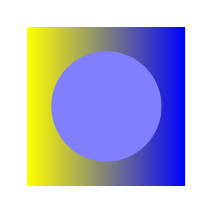
\begin{tikzpicture}[baseline=1cm]
\shade[left color=yellow,right color=blue!100] (0,0) rectangle (2,2);
\fill[blue!50] (1,1) circle (0.7);
\end{tikzpicture}
\\ \hline 
\parbox[c]{11cm}{ 
\ESS{begin\AC{tikzfadingfrompicture}}[\RDD{name}=tikz] \\
\BS{node} [draw,text=transparent!20] \\
\AC{\BS{fontfamily}\AC{ptm}\BS{fontsize}\AC{25}\AC{25}\BS{bfseries}\BS{selectfont} TikZ};\\
\ESS{end\AC{tikzfadingfrompicture}} }
& 

\begin{tikzpicture}[baseline=-.3cm]
\node [draw,text=transparent!20]
{\fontfamily{ptm}\fontsize{25}{25}\bfseries\selectfont TikZ};
\end{tikzpicture}
 \\ \hline 
\end{tabular} 

%\begin{tabular}{|c|c|c|} \hline  
\begin{tikzfadingfrompicture}[name=filtre]
\shade[left color=yellow,right color=blue!100] (0,0) rectangle (2,2);
\fill[blue!50] (1,1) circle (0.7);
\end{tikzfadingfrompicture}


\begin{tikzfadingfrompicture}[name=tikz]
\node [text=transparent!20]
{\fontfamily{ptm}\fontsize{25}{25}\bfseries\selectfont Ti\emph{k}Z};
\end{tikzfadingfrompicture}

\bigskip

\begin{tabular}{|c|c|} \hline 
\multicolumn{2}{|c|}{ \TFRGB{Utilisation dans un rectangle}{Use in a frame}}
 \\ \hline 
\multicolumn{2}{|c|}{\BS{fill}[\RDD{path fading}=filtre] (-2,-1) rectangle (2,1); }

\\ \hline 
\begin{tikzpicture}
\draw(-2,-1) rectangle (2,1);
\fill[path fading=filtre] (-2,-1) rectangle (2,1);
\end{tikzpicture}
&  
\begin{tikzpicture}
\draw(-2,-1) rectangle (2,1);
\fill[path fading=tikz] (-2,-1) rectangle (2,1);
\end{tikzpicture}
\\ \hline  
[\RDD{path fading}=filtre] &  [\RDD{path fading}=tikz]
\\ \hline 
\begin{tikzpicture}
\draw(-2,-1) rectangle (2,1);
\fill[path fading=filtre ,fit fading=false] (-2,-1) rectangle (2,1);
\end{tikzpicture}
&  
\begin{tikzpicture}
% Background
\draw(-2,-1) rectangle (2,1);
\fill[path fading=tikz,fit fading=false] (-2,-1) rectangle (2,1);
\end{tikzpicture}
\\ \hline 
[path fading=filtre ,\RDD{fit fading}=false] & [path fading=tikz,\RDD{fit fading}=false]
\\ 
\hline 
\begin{tikzpicture}
% Background
\draw(-2,-1) rectangle (2,1);
\fill[path fading=filtre ,left color=blue,right color=red] (-2,-1) rectangle (2,1);
\end{tikzpicture}
&  
\begin{tikzpicture}
\draw(-2,-1) rectangle (2,1);
\fill[path fading=tikz,left color=blue,right color=red] (-2,-1) rectangle (2,1);
\end{tikzpicture}
\\ \hline left color=blue,right color=red & [path left color=blue,right color=red  \\ 
\hline

\begin{tikzpicture}
 Background
\draw(-2,-1) rectangle (2,1);
\fill[path fading=filtre ,red] (-2,-1) rectangle (2,1);
\end{tikzpicture}
&  
\begin{tikzpicture}
 Background
\draw(-2,-1) rectangle (2,1);
\fill[path fading=tikz,red] (-2,-1) rectangle (2,1);
\end{tikzpicture}
\\ \hline 
[path fading=filtre ,red] &  [path fading=tikz,red] \\ 
\hline 
\end{tabular}
 
\bigskip


\begin{tabular}{|c|c|} \hline 
\multicolumn{2}{|c|}{\TFRGB{Utilisation dans un ellipse}{Use in an ellipse}}
 \\ \hline 
\multicolumn{2}{|c|}{\BS{fill}[\RDD{path fading}=filtre] (-2,-1) ellipse (2 and 1); }
\\ \hline
\begin{tikzpicture}
\draw  (-2,-1) ellipse (2 and 1);
\fill[path fading=filtre] (-2,-1) ellipse (2 and 1);
\end{tikzpicture}
&
\begin{tikzpicture}
\draw  (-2,-1) ellipse (2 and 1 );
\fill[path fading=tikz] (-2,-1) ellipse (2 and 1);
\end{tikzpicture}
\\ \hline
[\RDD{path fading}=filtre] &  [\RDD{path fading}=tikz]
\\ \hline
\end{tabular} 



%\subsection{Création de décoloration avec tikzfading}
\SbSSCT{Création de décoloration avec tikzfading}{Creating fading patterns with tikzfading}

\begin{tabular}{|c|c|} \hline
\parbox[c]{11cm}{ 
\BSS{tikzfading}[\RDD{name}={\color{purple} fade right},
left color=transparent!0,
right color=transparent!100]\\ \\
\BS{tikz} \BS{filldraw} [red,\RDD{path fading}={\color{purple} fade right}] (-1,-1) rectangle (1,1);}
&  
\tikzfading[name=fade right,
left color=transparent!0,
right color=transparent!100]

\tikz[baseline=0pt] \filldraw [red,path fading=fade right] (-1,-1) rectangle (1,1);
\\ \hline  
\parbox[c]{11cm}{ 
\BSS{tikzfading}[\RDD{name}={\color{purple}fade out},
inner color=transparent!0,
outer color=transparent!100]\\ \\
\BS{tikz} \BS{filldraw} [blue,\RDD{path fading}={\color{purple} fade out}] (-1,-1) rectangle (1,1);}
&  
\tikzfading[name=fade out,
inner color=transparent!0,
outer color=transparent!100]

\tikz[baseline=0pt] \filldraw [blue,path fading=fade out] (-1,-1) rectangle (1,1);

\\ \hline 
\parbox[c]{11cm}{ 
\BSS{tikzfading}[\RDD{name}={\color{purple}fade inside},
inner color=transparent!80,
outer color=transparent!10]\\ \\
\BS{tikz} \BS{filldraw} [blue,\RDD{path fading}={\color{purple} fade inside}] (-1,-1) rectangle (1,1);}
&  
\tikzfading[name=fade inside,
inner color=transparent!80,
outer color=transparent!10]

\tikz[baseline=0pt] \filldraw [blue,path fading= fade inside] (-1,-1) rectangle (1,1);
\\ \hline 
\parbox[c]{11cm}{ 
\BSS{tikzfading}[\RDD{name}={\color{purple}middle},
top color=transparent!80,
bottom color=transparent!80,
middle color=transparent!20]\\ \\
\BS{tikz} \BS{filldraw} [blue,\RDD{path fading}={\color{purple} middle}] (-1,-1) rectangle (1,1);}
&  
\tikzfading[name=middle,
top color=transparent!80,
bottom color=transparent!80,
middle color=transparent!20]

\tikz[baseline=0pt] \filldraw [blue,path fading= middle] (-1,-1) rectangle (1,1);

\\ \hline 
\end{tabular} 



%\subsubsection{Modification de la décoloration }
\SbSbSSCT{Modification de la décoloration }{Modification of the fading pattern}

\begin{center}
\RRR{23-4-2}
\end{center}

  
\begin{tabular}{|c|c|c|} \hline
\multicolumn{3}{|l|}{ \BS{fill} [blue,path fading=north,fading transform=\AC{yshift=-.5cm}] (-1,-1) rectangle (1,1);}
\\ \hline
\begin{tikzpicture}
 \draw (-1,-1) rectangle (1,1);
\fill [blue,path fading=north,fading transform={yshift=-.5cm}](-1,-1) rectangle (1,1);
\end{tikzpicture}
& 
\begin{tikzpicture}
 \draw (-1,-1) rectangle (1,1);
\fill [blue,path fading=north,fading transform={rotate=30}](-1,-1) rectangle (1,1);
\end{tikzpicture}
&
\begin{tikzpicture}
 \draw (-1,-1) rectangle (1,1);
\fill [blue,path fading=north,fading angle=30](-1,-1) rectangle (1,1);
\end{tikzpicture}
\\ \hline 
\RDD{fading transform}=\AC{yshift=-.5cm} & \RDD{fading transform}=\AC{yshift=-.5cm} & \RDD{fading angle}=30
\\ \hline 
\end{tabular} 

\bigskip

\begin{center}
\RRR{23-4-3}
\end{center}

\begin{tabular}{|c|c|} \hline
\parbox[b]{10cm}{
 \BS{begin}\AC{tikzpicture} \\
 \BS{draw}  (-1,-1) rectangle (1,1);\\
 \BS{path} [\RDD{scope fading}=east] (-1,-1) rectangle (1,1);\\
 \BS{fill}[red] ( 90:1) circle (1);\\
 \BS{fill}[green] (210:1) circle (1);\\
 \BS{fill}[blue] (330:1) circle (1); \\
 \BS{end}\AC{tikzpicture} \\
  }
&
 \begin{tikzpicture}
 \draw  (-1,-1) rectangle (1,1);
 \path [scope fading=east] (-1,-1) rectangle (1,1);
 \fill[red] ( 90:1) circle (1);
 \fill[green] (210:1) circle (1);
 \fill[blue] (330:1) circle (1);
 \end{tikzpicture}
 \\ \hline 
\end{tabular}


\bigskip
\begin{tabular}{|c|c|} \hline
\parbox[c]{8cm}{
\BS{tikz} \BS{node} [black,\RDD{scope fading}=south,fading angle=45,text width=5cm] \\
\AC{
VisualTIKZ VisualTIKZ VisualTIKZ VisualTIKZ VisualTIKZ VisualTIKZ VisualTIKZ VisualTIKZ VisualTIKZ VisualTIKZ VisualTIKZ VisualTIKZ VisualTIKZ 
}; 
 }
&
\tikz \node [black,scope fading=south,fading angle=45,text width=5cm]
{
VisualTIKZ VisualTIKZ VisualTIKZ VisualTIKZ VisualTIKZ VisualTIKZ VisualTIKZ VisualTIKZ VisualTIKZ VisualTIKZ VisualTIKZ VisualTIKZ VisualTIKZ 
};
 \\ \hline 
\end{tabular}

%%=========================

\subsection{Transparency Groups} 

\begin{center}
\RRR{23-5}
\end{center}

\begin{tabular}{|c|c|} \hline 
\multicolumn{2}{|l|}{\BS{begin}\AC{tikzpicture}[opacity=.5]} \\
\multicolumn{2}{|l|}{ \BS{draw} [line width=1cm] (0,0) -- (2,2); }\\
\multicolumn{2}{|l|}{ \BS{draw} [line width=1cm] (0,2) -- (2,0); }\\
\multicolumn{2}{|l|}{\BS{end}\AC{tikzpicture}}
 \\ \hline 
\begin{tikzpicture}[opacity=.5]
\draw [line width=1cm] (0,0) -- (2,2);
\draw [line width=1cm] (0,2) -- (2,0);
\end{tikzpicture}
& 
\begin{tikzpicture}[opacity=.5,transparency group]
\draw [line width=1cm] (0,0) -- (2,2);
\draw [line width=1cm] (0,2) -- (2,0);
\end{tikzpicture} 
 \\ 
\hline [opacity=.5] & [opacity=.5,\RDD{transparency group}] \\ 
\hline 
\end{tabular} 

\bigskip

\begin{tabular}{|c|c|} \hline 
\multicolumn{2}{|c|}{\TFRGB{A revoir : ne fonctionne pas}{Not working !} }
\\ \hline  
\parbox[c]{9cm}{ 
\BS{begin}\AC{tikzpicture} \\
\BS{shade} [left color=red,right color=blue] (-2,-1) rectangle (2,1); \\
\BS{begin}\AC{scope}[transparency group=knockout] \\
\BS{fill]}[white] (-1.9,-.9) rectangle (1.9,.9); \\
\BS{node} [opacity=0] {TikZ}; \\
\BS{end}\AC{scope} \\
\BS{end}\AC{tikzpicture}
}
&  
\begin{tikzpicture}[baseline=0pt]
\shade [left color=red,right color=blue] (-2,-1) rectangle (2,1);
\fill [white] (-1.9,-.9) rectangle (1.9,.9);
\node [opacity=0,transparency group=knockout]{TikZ};
\end{tikzpicture}
\\ \hline 
\end{tabular} 

